% =====================================================================
% Artigo - Projeto Final de FGA0315 Qualidade de Software 1 (2026/2)
% Equipe Adele Goldstine - Turma T02
%
% Modelo: IEEEtran v1.8b para conferências (bare_conf.tex), obtido no
% CTAN (https://ctan.org/pkg/ieeetran). O modelo original, sem alterações,
% está em modelo-ieee/. Compilação: ver README.md.
%
% Conforme orientação da professora, o artigo não tem capa nem sumário:
% começa direto no título, autores, resumo e Introdução, como no modelo
% do IEEE.
% =====================================================================
\documentclass[conference,a4paper]{IEEEtran}

\usepackage{iftex}
\ifXeTeX
	% XeLaTeX/Tectonic: equivalentes OpenType das fontes do IEEEtran
	% (Times, Helvetica e Courier)
	\usepackage{fontspec}
	\setmainfont{texgyretermes}[Extension=.otf, UprightFont=*-regular,
		BoldFont=*-bold, ItalicFont=*-italic, BoldItalicFont=*-bolditalic]
	\setsansfont{texgyreheros}[Extension=.otf, UprightFont=*-regular,
		BoldFont=*-bold, ItalicFont=*-italic, BoldItalicFont=*-bolditalic]
	\setmonofont{texgyrecursor}[Extension=.otf, UprightFont=*-regular,
		BoldFont=*-bold, ItalicFont=*-italic, BoldItalicFont=*-bolditalic]
\else
	\usepackage[T1]{fontenc}
	\usepackage[utf8]{inputenc}
\fi
\usepackage[brazil]{babel}
\usepackage{cite}
\usepackage{amsmath}
\usepackage{graphicx}
\usepackage{array}
\usepackage{booktabs}
\usepackage{tabularx}
\usepackage[table]{xcolor}
\usepackage{tikz}
\usetikzlibrary{arrows.meta,positioning}
\usepackage{url}
\usepackage[hidelinks]{hyperref}

% Colunas com quebra de linha e alinhamento à esquerda
\newcolumntype{L}[1]{>{\raggedright\arraybackslash}p{#1}}
\newcolumntype{C}[1]{>{\centering\arraybackslash}p{#1}}
\newcolumntype{Y}{>{\raggedright\arraybackslash}X}

% Fonte de tabelas e figuras (exigida pelos critérios da disciplina)
\newcommand{\fonte}[1]{\par\vspace{2pt}{\footnotesize Fonte: #1}}

\newcommand{\repositorio}{\url{https://github.com/FCTE-Qualidade-de-Software-1/2026-2_T02_ADELE_GOLDSTINE}}
\newcommand{\gitpage}{\url{https://fcte-qualidade-de-software-1.github.io/2026-2_T02_ADELE_GOLDSTINE/}}

\renewcommand{\IEEEkeywordsname}{Palavras-chave}

\hyphenation{SIGAA Ca-pa-ci-da-de Fle-xi-bi-li-da-de por-ta-bi-li-da-de}

\begin{document}

\title{Avaliação da Qualidade do SIGAA/UnB na\\Perspectiva do Estudante de Graduação}

\author{\IEEEauthorblockN{Arthur Carvalho Leite, Caio Melo Borges, Daniel Nunes Duarte,\\
Davi dos Santos Brito Nobre, Felipe de Aquino Campêlo e Leonardo Fachinello Bonetti}
\IEEEauthorblockA{Equipe Adele Goldstine -- FGA0315 Qualidade de Software 1, Turma T02 -- Profa. Cristiane Soares Ramos\\
Faculdade de Ciências e Tecnologias em Engenharia (FCTE), Universidade de Brasília (UnB), Brasília, DF\\
Repositório: \repositorio}}

\maketitle

\begin{abstract}
O Sistema Integrado de Gestão de Atividades Acadêmicas (SIGAA) é o ponto único de acesso do estudante da Universidade de Brasília (UnB) a notas, horários, histórico, documentos e turmas virtuais. Relatos de dificuldade de uso, uma interface pensada para computador de mesa e ferramentas comunitárias que suprem funções do sistema motivam uma avaliação objetiva da sua qualidade. Este artigo apresenta a especificação dessa avaliação, segundo o processo de avaliação da família SQuaRE (ISO/IEC 25040) e o modelo de qualidade da ISO/IEC 25010:2023. Na Fase 1, uma matriz Impacto~$\times$~Risco com filtro de viabilidade priorizou quatro características, e personas deram concretude aos perfis de usuários. Por orientação recebida no ponto de controle, a especificação concentra-se em três delas: Capacidade de Interação (Usabilidade), Adequação Funcional e Flexibilidade (Portabilidade). Na Fase 2, o método \textit{Goal-Question-Metric} (GQM) as desdobrou em três objetivos, 12 questões com hipóteses e 16 métricas, com níveis de pontuação e critérios de julgamento fixados antes da coleta. A especificação combina teste com usuários, inspeção por dois avaliadores, verificação automática de acessibilidade e um questionário que compara estudantes de diferentes semestres. A gestão do projeto é acompanhada por indicadores do PSM/CID.
\end{abstract}

\begin{IEEEkeywords}
qualidade de produto de software, SQuaRE, ISO/IEC 25010, GQM, PSM, SIGAA.
\end{IEEEkeywords}

\section{Introdução}
\label{sec:introducao}

O Sistema Integrado de Gestão de Atividades Acadêmicas (SIGAA), desenvolvido pela Universidade Federal do Rio Grande do Norte (UFRN) e adotado por diversas universidades federais, é o sistema pelo qual o estudante de graduação da Universidade de Brasília (UnB) consulta notas, horários, histórico e índices acadêmicos, emite documentos, realiza matrícula e acessa as turmas virtuais \cite{sigaa}. Não há alternativa institucional: uma dificuldade no sistema se converte em atraso, erro de planejamento ou dependência de colegas e de ferramentas de terceiros.

Há indícios de que o SIGAA não atende bem esse público. A interface foi concebida para computador de mesa, com largura fixa e menus que se abrem pela passagem do ponteiro do mouse; o horário das turmas aparece em notação codificada (``24M34''); e estudantes recorrem a ferramentas criadas pela comunidade para planejar o fluxo de disciplinas. Esses indícios, porém, são percepções. Para apoiar decisões de melhoria, precisam ser transformados em evidências mensuráveis e comparadas a critérios definidos antes da coleta.

A família SQuaRE oferece o arcabouço para essa transformação: um modelo de qualidade \cite{iso25010_2023}, um catálogo de medidas \cite{iso25023} e um processo de avaliação \cite{iso25040}. O método \textit{Goal-Question-Metric} (GQM) liga os objetivos às questões e às métricas \cite{basili1994}, e o \textit{Practical Software and Systems Measurement} (PSM) orienta a medição do próprio projeto \cite{mcgarry2002}.

O objetivo geral é \textbf{avaliar a qualidade do portal do discente de graduação do SIGAA/UnB, do ponto de vista do estudante}, para identificar com evidências os pontos fracos nas tarefas mais frequentes e apoiar a priorização de melhorias pela Secretaria de Tecnologia da Informação (STI/UnB). Os objetivos específicos são: (i) estabelecer os requisitos da avaliação (Fase 1); (ii) especificá-la pelo GQM, com métricas, níveis de pontuação e critérios de julgamento (Fase 2); (iii) projetá-la e executá-la, julgando os resultados e as relações entre as características (Fases 3 e 4); e (iv) executar uma ação de melhoria baseada nas evidências. Este artigo corresponde à Entrega 1 e cobre os itens (i) e (ii) \cite{ramos2026roteiro}.

A Seção~\ref{sec:referencial} apresenta o referencial teórico; a Seção~\ref{sec:metodologia}, a metodologia e a gestão do projeto; as Seções~\ref{sec:fase1} e~\ref{sec:fase2}, as Fases 1 e 2; e a Seção~\ref{sec:consideracoes}, as considerações parciais. A contribuição da equipe está no Apêndice~\ref{ap:contribuicao}. Os artefatos citados (páginas detalhadas, dados, instrumentos e histórico de versões) estão no repositório da equipe\footnote{\repositorio} e na página do projeto\footnote{\gitpage}.

\section{Referencial teórico}
\label{sec:referencial}

\subsection{Qualidade de produto e a família SQuaRE}
\label{sec:square}

A série ISO/IEC 25000 (SQuaRE) organiza os requisitos, modelos, medidas e o processo de avaliação da qualidade de sistemas e software \cite{iso25000}. A ISO/IEC 25010:2023 substitui a versão de 2011 e organiza a qualidade do produto em nove características \cite{iso25010_2023}: Adequação Funcional, Eficiência de Desempenho, Compatibilidade, Capacidade de Interação (Usabilidade, em 2011), Confiabilidade, Segurança, Manutenibilidade, Flexibilidade (Portabilidade, em 2011) e Segurança Operacional (nova). Neste texto, as características renomeadas aparecem com o nome de 2023 seguido do de 2011. A satisfação integrava o modelo de qualidade em uso da versão de 2011 \cite{iso25010_2011} e, quando usada, é tratada como medida complementar de qualidade em uso \cite{iso25022}.

\subsection{Processo de avaliação de produto}
\label{sec:processo}

A ISO/IEC 25040 descreve a avaliação como um processo em atividades sucessivas \cite{iso25040}. No material da disciplina, ele é apresentado em quatro fases \cite{ramos2026processo}: (1) estabelecer os requisitos (propósito, tipo de produto e modelo de qualidade); (2) especificar a avaliação (métricas, níveis de pontuação e critérios de julgamento); (3) projetar a avaliação (plano com método, instruções, recursos e cronograma); e (4) executá-la (obter as medidas, compará-las com os critérios e julgar). A especificação deve ser detalhada o bastante para que a avaliação seja repetível e reprodutível. As Fases 1 e 2 formam a Entrega 1, e as Fases 3 e 4, a Entrega 2 \cite{ramos2026roteiro}.

\subsection{Método Goal-Question-Metric}
\label{sec:gqm}

O GQM parte do princípio de que a medição deve ser orientada a objetivos \cite{basili1994}. A definição ocorre em três níveis: \textbf{conceitual} (objetivo), \textbf{operacional} (questões que caracterizam o objeto quanto ao foco de qualidade) e \textbf{quantitativo} (métricas que respondem às questões); a interpretação segue o caminho inverso \cite{ramos2026gqm}. Cada objetivo é escrito em um \textit{template} com objeto, propósito, foco de qualidade, ponto de vista e contexto \cite{basili1994}, e cada questão recebe uma hipótese, a resposta esperada antes da medição. Boas métricas são simples, objetivas, fáceis de coletar, robustas e válidas \cite{ramos2026gqm}.

\subsection{Medição prática de software e sistemas}
\label{sec:psm}

O PSM é uma abordagem de medição dirigida por necessidades de informação e ligada à gestão de projetos \cite{mcgarry2002}. Seu modelo de informação, adotado pela ISO/IEC/IEEE 15939 \cite{iso15939}, liga atributos a medidas básicas, medidas derivadas e indicadores, estes associados a critérios de decisão \cite{ramos2026psm}. As necessidades de informação são agrupadas em categorias, entre elas calendário e progresso, recursos e custos e desempenho dos processos. O \textit{framework} CID adapta essas categorias a equipes que trabalham em ciclos curtos, com medidas como \textit{burndown}, comprometido \textit{versus} concluído e tempo de ciclo \cite{psmcid1,psmcid2}.

\subsection{Medidas de referência}
\label{sec:medidas-referencia}

A ISO/IEC 25023 define medidas de produto como cobertura e correção funcional na forma $X = 1 - A/B$ \cite{iso25023}, e a ISO/IEC 25022, medidas de eficácia, eficiência e satisfação em uso \cite{iso25022}. A taxa de conclusão de tarefas tem média de referência de 78\% \cite{sauro2011}. O \textit{System Usability Scale} (SUS) produz uma pontuação de 0 a 100 \cite{brooke1996}, com média de referência 68 \cite{sauro2016}, e a \textit{Single Ease Question} (SEQ) mede a facilidade percebida de uma tarefa em um item \cite{sauro2016}. A acessibilidade é verificada pelos critérios A e AA das WCAG~2.2 \cite{wcag22}.

\subsection{Personas}
\label{sec:personas-ref}

Personas são arquétipos de usuários, descritos com objetivos, contexto e frustrações, que orientam o projeto e a avaliação de um produto para quem de fato o usa \cite{cooper1999}. A antipersona descreve quem não é público-alvo e ajuda a delimitar o escopo. Em uma avaliação de qualidade, as personas tornam concreto o ponto de vista declarado nos objetivos de medição e ajudam a escolher tarefas e recortes de análise.

\section{Metodologia de desenvolvimento do projeto}
\label{sec:metodologia}

\subsection{Processo e organização do trabalho}

A avaliação segue as quatro fases do processo de avaliação de produto (Seção~\ref{sec:processo}). A equipe atua como \textbf{avaliador independente}: não desenvolve nem opera o SIGAA e não tem acesso a código-fonte ou infraestrutura, o que torna a avaliação externa (caixa-preta).

O trabalho é organizado no repositório Git da disciplina. Cada fase é desenvolvida em um ramo próprio (\texttt{fase-1}, \texttt{fase-2}, \texttt{artigo-latex}) e integrada ao ramo principal por \textit{pull request} (PR), após revisão por outro membro. Os \textit{commits} recebem um identificador de tarefa (\texttt{[D01]} a \texttt{[D09]} na Entrega 1), que permite rastrear cada alteração até a atividade de origem. A documentação é publicada automaticamente como GitPage (MkDocs), e cada página traz histórico de versões com data, descrição e autor. As decisões são tomadas em reunião: cada membro elabora sua proposta, as propostas são consolidadas e as divergências discutidas até o consenso, como na matriz Impacto~$\times$~Risco (Seção~\ref{sec:priorizacao}).

\subsection{Gestão do projeto com indicadores PSM/CID}
\label{sec:gestao}

O roteiro exige acompanhar o projeto com métricas do PSM/CID nas categorias calendário e progresso, recursos e custos e desempenho dos processos \cite{ramos2026roteiro}. A Tabela~\ref{tab:psm} apresenta os indicadores, construídos segundo o modelo de informação do PSM \cite{mcgarry2002} e adaptados do \textit{framework} CID \cite{psmcid2}, com a primeira medição, feita em 19/10/2026 a partir do histórico do repositório, a sete dias da entrega. O procedimento de extração e os dados estão na página de gestão da GitPage.

As decisões da Tabela~\ref{tab:psm} começaram a ser aplicadas antes da entrega. Para o I3, a equipe adotou a planilha de esforço em horas-pessoa (\texttt{gestao/esforco.csv}), com um \textit{script} versionado que soma as horas e calcula a participação de cada membro (\texttt{gestao/esforco.py}). As horas da Entrega 1 foram reconstruídas por estimativa, e todos os membros ficaram entre 13,9\% e 18,8\%, dentro do critério de decisão (Apêndice~\ref{ap:contribuicao}). A partir da Entrega 2, as horas são registradas por atividade e revisadas pela equipe.

\begin{table*}[!t]
	\caption{Indicadores PSM/CID para a gestão do projeto e primeira medição (19/10/2026)}
	\label{tab:psm}
	\centering
	\footnotesize
	\begin{tabularx}{\textwidth}{L{1.6cm} L{3.9cm} L{3.4cm} L{3.0cm} Y}
		\toprule
		\textbf{Categoria} & \textbf{Indicador (medidas)} & \textbf{Critério de decisão} & \textbf{Valor medido} & \textbf{Interpretação e decisão} \\
		\midrule
		Calendário e progresso & \textbf{I1} Comprometido \textit{vs.} concluído: artefatos da entrega integrados ao ramo principal / planejados & $<$80\% a uma semana da entrega exige redistribuição de tarefas & 14 de 17 (82\%): 14 páginas das Fases 1 e 2; artigo, contribuição e \textit{release} pendentes & Dentro do critério. Priorizar o artigo e a tabela de contribuição \\
		& \textbf{I2} \textit{Burndown}: \textit{issues} abertas do marco da entrega, por dia & Desvio $>$10\% da linha planejada é discutido em reunião & Não mensurável: nenhuma \textit{issue} ou marco & Lacuna de processo. Criar marcos E1 e E2 e uma \textit{issue} por artefato \\
		Recursos e custos & \textbf{I3} Esforço por membro: horas na planilha de esforço e participação (\%) & Participação $<$10\% ou $>$40\% exige rebalanceamento & Planilha não adotada; \textit{proxy}: \textit{commits} por membro = 9, 3, 3, 2 e 0 & \textit{Commits} não medem esforço. Adotar a planilha, que alimenta a tabela de contribuição \\
		Desempenho dos processos & \textbf{I4} Tempo de ciclo: primeiro \textit{commit} do ramo até a integração do PR (h) & Ciclo $>$5 dias indica integração tardia & Fase 1: 49,0~h; Fase 2: 16,7~h & Dentro do critério. Manter um ramo e um PR por fase \\
		& \textbf{I5} Retrabalho: correções após revisão / alterações do PR (\%) & $>$30\% motiva \textit{checklist} de revisão & Não medido: revisões não registradas & Registrar a revisão nos PRs a partir da Fase 3 \\
		\bottomrule
	\end{tabularx}
	\fonte{elaborado pela equipe, com base em \cite{mcgarry2002,psmcid2} e no histórico do repositório.}
\end{table*}

\subsection{Aspectos éticos e rastreabilidade}

Nenhuma tarefa altera dados acadêmicos: todas são consultas ou emissões de documentos feitas pelos participantes com as próprias credenciais. A participação em testes e no questionário é voluntária e precedida de termo de consentimento, e as sessões só são gravadas mediante consentimento \cite{ramos2026roteiro}. Os participantes são identificados por código (P1, P2, \ldots) e perfil, e capturas de tela têm os dados pessoais ocultados. Os dados brutos anonimizados, os consolidados e os procedimentos de cálculo ficarão na pasta \texttt{dados/} do repositório; as gravações terão acesso restrito à equipe e à professora.

\subsection{Declaração de uso de inteligência artificial}

A equipe usou o Claude Opus 5.5 (Claude Code) para: (a) apoiar a redação e a formatação das páginas da Fase 1; (b) apoiar a redação da Fase 2 e verificar a consistência entre as páginas e o roteiro; (c) pesquisar as características de qualidade oficiais e padronizadas da ISO/IEC 25010 e a padronização do IEEE (modelo IEEEtran) para a documentação em LaTeX; (d) propor a metodologia de esforço por horas e o \textit{script} de cálculo; e (e) atualizar o artigo após os ajustes da Fase 2 e a inclusão das personas. O DeepSeek v4 foi usado na estruturação inicial do repositório. Todo conteúdo gerado foi conferido pela equipe contra as páginas do repositório e o roteiro; as referências foram verificadas uma a uma, e os números citados foram conferidos com as fontes originais. O registro completo está na página de uso de IA da GitPage.

\section{Fase 1: requisitos da avaliação}
\label{sec:fase1}

\subsection{Propósito e partes interessadas}

O propósito é \textbf{identificar, com evidências mensuráveis, os pontos fracos do SIGAA nas tarefas acadêmicas mais frequentes do estudante de graduação}, para apoiar a priorização de melhorias pela STI/UnB e embasar a ação de melhoria da Fase 4. O ponto de vista é o do estudante, com atenção a perfis vulneráveis: calouros, que desconhecem a terminologia acadêmica; estudantes que acessam o sistema apenas pelo celular; e estudantes com deficiência. Veteranos e formandos servem de contraste: problemas que persistem com experiência indicam falhas de operabilidade.

A demanda parte da disciplina FGA0315, que define o processo e os critérios de aceitação. Os resultados destinam-se à STI/UnB, operadora do sistema, que decidirá quais telas e fluxos priorizar (pelo ranking das tarefas), se investe em interface responsiva (pela Flexibilidade cruzada com o perfil de acesso) e se otimiza páginas específicas (pelo desempenho por página); ao Decanato de Ensino de Graduação e às coordenações, que decidirão quais procedimentos precisam de orientação (pelas tarefas com mais erro ou abandono); à comunidade estudantil; e à UFRN, desenvolvedora do produto.

\subsection{Produto avaliado}
\label{sec:produto}

O objeto é o \textbf{portal do discente de graduação do SIGAA/UnB}, versão v4.15.10.115 (rodapé do sistema em 16/10/2026), acessado pela interface web em produção (Fig.~\ref{fig:portal}) \cite{sigaa}. É um sistema de informação web, transacional e institucional, em JavaServer Faces, acessado pela Autenticação Integrada dos sistemas SIG. Pela classificação da IEEE 1062 apresentada na disciplina, é um produto MOTS (\textit{Modified Off-The-Shelf}): um produto-padrão da UFRN implantado com configurações próprias por instituição \cite{ramos2026processo}. Por ser de código fechado, a avaliação se restringe ao comportamento observável: é possível medir tempo de carregamento no navegador, conclusão e esforço nas tarefas, comportamento em navegadores e telas e acessibilidade, mas não o processamento no servidor, o comportamento sob carga ou a qualidade do código.

\begin{figure}[!t]
	\centering
	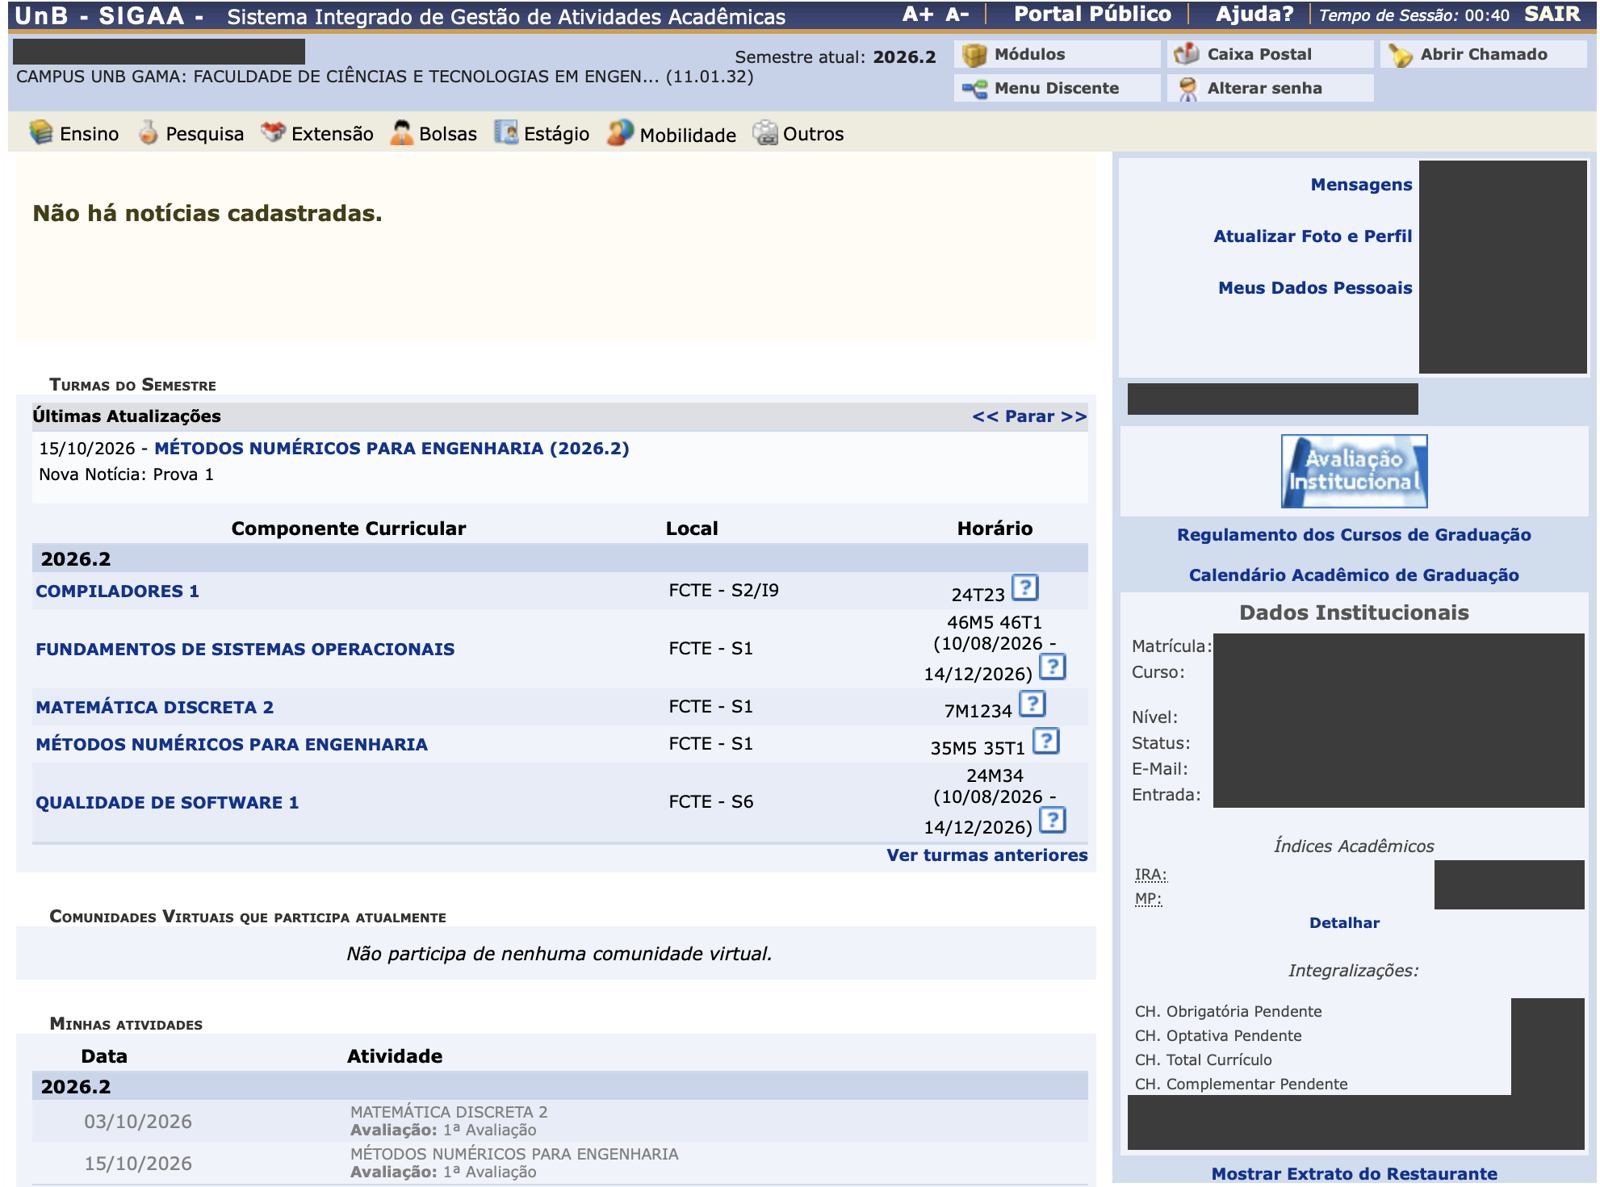
\includegraphics[width=\columnwidth]{figuras/sigaa-portal-discente.png}
	\caption{Página inicial do portal do discente do SIGAA/UnB.}
	\label{fig:portal}
	\fonte{captura da equipe em 16/10/2026, com dados pessoais ocultados.}
\end{figure}

A inspeção inicial produziu oito observações preliminares (OP), que não são resultados, mas indícios que orientaram a seleção das características (Tabela~\ref{tab:op}).

\begin{table}[!t]
	\caption{Observações preliminares da interface}
	\label{tab:op}
	\centering
	\footnotesize
	\begin{tabularx}{\columnwidth}{L{0.75cm} Y L{2.4cm}}
		\toprule
		\textbf{ID} & \textbf{Observação} & \textbf{Característica} \\
		\midrule
		OP-01 & Horários em notação codificada (``24M34''), legível só com legenda & Cap. Interação (autodescritividade) \\
		OP-02 & Menus abertos pela passagem do ponteiro, sem equivalente para toque & Flexibilidade; Cap. Interação \\
		OP-03 & Layout de largura fixa & Flexibilidade \\
		OP-04 & Menu Ensino com cerca de 20 itens em um nível & Cap. Interação (reconhecimento) \\
		OP-05 & Duas estruturas de navegação (portal e Turma Virtual) & Cap. Interação (operabilidade) \\
		OP-06 & Sessão que expira por inatividade & Cap. Interação (proteção contra erros) \\
		OP-07 & Ferramentas comunitárias para planejar o fluxo de disciplinas & Adequação Funcional (completude) \\
		OP-08 & Ampliação de fonte (A+/A-) no cabeçalho (ponto positivo) & Cap. Interação (inclusividade) \\
		\bottomrule
	\end{tabularx}
	\fonte{elaborado pela equipe.}
\end{table}

\subsection{Modelo de qualidade e priorização}
\label{sec:priorizacao}

O modelo da ISO/IEC 25010:2023 foi adaptado por três filtros: relevância para as partes interessadas, mensurabilidade em avaliação caixa-preta e viabilidade ética (nenhum teste pode alterar dados reais ou sobrecarregar a produção). Para escolher de três a quatro características, cada membro atribuiu notas de 1 a 5 de \textbf{impacto} ($I$), a consequência de uma deficiência, e de \textbf{risco} ($R$), a probabilidade de deficiência estimada pelas OP, pela idade da tecnologia e por relatos dos estudantes. A prioridade é $P = I \times R$, e foram selecionadas as características viáveis com $P \geq 15$ (Tabela~\ref{tab:matriz}).

\begin{table}[!t]
	\caption{Matriz Impacto $\times$ Risco}
	\label{tab:matriz}
	\centering
	\footnotesize
	\begin{tabularx}{\columnwidth}{L{2.25cm} C{0.2cm} C{0.2cm} C{0.35cm} Y}
		\toprule
		\textbf{Característica} & $I$ & $R$ & $P$ & \textbf{Decisão} \\
		\midrule
		Cap. de Interação & 5 & 5 & \textbf{25} & Selecionada (1): seis das oito OP \\
		Adequação Funcional & 5 & 4 & \textbf{20} & Selecionada (2): dados afetam decisões (OP-07) \\
		Efic. de Desempenho & 4 & 4 & \textbf{16} & Selecionada (3): pesa em rede móvel \\
		Flexibilidade & 4 & 4 & \textbf{16} & Selecionada (4): OP-02 e OP-03 \\
		Confiabilidade & 4 & 3 & 12 & Preterida: falhas na matrícula, fora da coleta \\
		Segurança & 5 & 2 & 10 & Inviável: exigiria testes de invasão \\
		Manutenibilidade & 3 & 3 & 9 & Inviável: sem código-fonte \\
		Compatibilidade & 2 & 2 & 4 & Preterida: não observável \\
		Seg. Operacional & 1 & 1 & 1 & Não se aplica \\
		\bottomrule
	\end{tabularx}
	\fonte{elaborado pela equipe.}
\end{table}

Nas características selecionadas, foram removidas as subcaracterísticas não mensuráveis no contexto: engajamento e assistência ao usuário (Capacidade de Interação), capacidade (Eficiência de Desempenho, por exigir testes de carga) e instalabilidade, substituibilidade e escalabilidade (Flexibilidade). O custo dessa seleção é que a avaliação descreve a qualidade do sistema em uso pelo estudante, e não a robustez interna da implementação.

\subsection{Escopo, tarefas e rigor}
\label{sec:escopo}

A avaliação usa seis tarefas representativas, escolhidas por frequência, criticidade e disponibilidade na coleta (Tabela~\ref{tab:tarefas}), executadas nos navegadores Chrome, Firefox, Safari e Edge, em telas de cerca de 360, 768 e 1280~px, e em rede comum e móvel simulada.

\begin{table}[!t]
	\caption{Tarefas representativas}
	\label{tab:tarefas}
	\centering
	\footnotesize
	\begin{tabularx}{\columnwidth}{C{0.35cm} Y L{2.7cm}}
		\toprule
		\textbf{ID} & \textbf{Tarefa} & \textbf{Caminho no sistema} \\
		\midrule
		T1 & Consultar as notas de uma disciplina & Ensino $>$ Consultar Notas \\
		T2 & Identificar dia, horário e local de uma turma & Página inicial $>$ Turmas \\
		T3 & Emitir atestado de matrícula ou histórico & Ensino $>$ Emitir Atestado \\
		T4 & Verificar índices e carga horária pendente & Ensino $>$ Índices Acadêmicos \\
		T5 & Acessar material na Turma Virtual & Turma Virtual $>$ Materiais \\
		T6 & Consultar o calendário acadêmico & Ensino $>$ Calendário \\
		\bottomrule
	\end{tabularx}
	\fonte{elaborado pela equipe.}
\end{table}

Ficam fora do escopo os portais de docentes e servidores, a pós-graduação, matrícula e trancamento (que alterariam dados reais), os demais sistemas SIG e os testes de carga e de segurança. O rigor é \textbf{intermediário}: a avaliação apoia decisões de priorização, sem impacto sobre segurança ou finanças, e é garantido por métricas objetivas, critérios fixados antes da coleta, medições repetidas e dois avaliadores nas inspeções. A amostra de conveniência, concentrada na FCTE, a versão do sistema e o período de coleta são declarados como limites de validade. A avaliação também se relaciona às metas 4.3, 10.2 e 16.6 dos Objetivos de Desenvolvimento Sustentável \cite{onu2015,ipea2018}: a permanência no ensino superior depende do sistema, estudantes de menor renda dependem mais do celular e de redes móveis, e o indicador 16.6.2 mede a satisfação com serviços públicos.

\section{Fase 2: especificação da avaliação}
\label{sec:fase2}

A Fase 2 seleciona as métricas e estabelece os níveis de pontuação e os critérios de julgamento \cite{iso25040,ramos2026processo}, pelo método GQM \cite{basili1994}. Cada métrica tem definição, cálculo, fonte dos dados, procedimento de coleta e interpretação documentados na GitPage; esta seção apresenta a síntese.

\subsection{Rastreabilidade com a Fase 1}

Todos os elementos do GQM derivam de decisões da Fase 1: as quatro características priorizadas originam os objetivos G1 a G4; as subcaracterísticas mantidas originam as questões; o ponto de vista e os perfis definem os recortes de análise (por perfil em M5, M6, M7 e M11; celular em Q12; questionário por semestre); as observações preliminares fundamentam as hipóteses (OP-01 em M11, OP-02 e OP-03 em M14, OP-04 em M4, OP-05 em M6 e M7, OP-06 em M8 e M20, OP-07 em M1 e M3); as decisões apoiadas definem a forma dos resultados (ranking das tarefas, G3 para a interface responsiva, M16 a M19 por página); e o rigor intermediário define dois avaliadores em M1, M2, M10 e M20 e cinco execuções em M16 a M19.

\subsection{Objetivos de medição}

Cada objetivo segue o \textit{template} GQM (Tabela~\ref{tab:objetivos}). Em todos, o propósito é \textbf{avaliar, a fim de identificar pontos fracos}, do ponto de vista do \textbf{estudante de graduação da UnB}, com o recorte indicado. Os resultados serão apresentados na ordem de prioridade da Fase 1: G2, G1, G4 e G3.

\begin{table*}[!t]
	\caption{Objetivos de medição no template GQM}
	\label{tab:objetivos}
	\centering
	\footnotesize
	\begin{tabularx}{\textwidth}{L{2.1cm} Y Y Y Y}
		\toprule
		& \textbf{G1 -- Adequação Funcional} & \textbf{G2 -- Capacidade de Interação} & \textbf{G3 -- Flexibilidade} & \textbf{G4 -- Eficiência de Desempenho} \\
		\midrule
		\textbf{Analisar} & o portal do discente do SIGAA/UnB & a interface web do portal do discente & a interface web do portal do discente & as páginas das tarefas T1 a T6 \\
		\textbf{Com respeito à} & completude, correção e pertinência funcional & reconhecimento de adequação, apreensibilidade, operabilidade, proteção contra erros, inclusividade, autodescritividade e satisfação & adaptabilidade a navegadores, telas e toque & comportamento temporal e utilização de recursos no cliente \\
		\textbf{Recorte do ponto de vista} & estudante de graduação & calouros e pessoas com deficiência & quem acessa só pelo celular & quem acessa por rede móvel \\
		\textbf{Contexto} & T1 a T6 e planejamento do fluxo; v4.15.10.115, 2026/2 & execução de T1 a T6 em computador & Chrome, Firefox, Edge e Safari; computador, tablet e celular & medição no cliente, em rede comum e móvel simulada \\
		\bottomrule
	\end{tabularx}
	\fonte{elaborado pela equipe.}
\end{table*}

\subsection{Questões e hipóteses}

Cada questão caracteriza um atributo do foco de qualidade e recebe uma hipótese com critério de confirmação numérico, declarado antes da coleta (Tabela~\ref{tab:questoes}). Na Fase 4, cada hipótese será classificada como confirmada, refutada ou inconclusiva; uma hipótese refutada indica que a percepção da Fase 1 não se confirmou.

\begin{table*}[!t]
	\caption{Questões, atributos e hipóteses}
	\label{tab:questoes}
	\centering
	\footnotesize
	\begin{tabularx}{\textwidth}{L{0.5cm} L{5.4cm} L{2.9cm} Y}
		\toprule
		\textbf{ID} & \textbf{Questão} & \textbf{Atributo} & \textbf{Hipótese (critério de confirmação)} \\
		\midrule
		Q1 & O SIGAA oferece as funções de que o estudante precisa? & Completude & H1: cobertura entre 75\% e 90\%, pior em T4 e no planejamento do fluxo (M1 Regular) \\
		Q2 & As informações exibidas estão corretas? & Correção & H2: nenhuma divergência com as fontes oficiais (M2 = 100\%) \\
		Q3 & As funções bastam para planejar o fluxo sem ferramentas externas? & Pertinência & H3: 25\% a 50\% dos respondentes usam ferramenta externa (M3 Regular) \\
		\midrule
		Q4 & O estudante identifica onde está a função? & Reconhecimento de adequação & H4: 50\% a 75\% de acerto na primeira escolha de menu (M4 Regular) \\
		Q5 & Conclui as tarefas sem ajuda, inclusive no primeiro contato? & Apreensibilidade & H5: conclusão geral de 78\% a 90\% (M5 Bom), mas abaixo de 65\% entre calouros \\
		Q6 & A navegação evita esforço desnecessário? & Operabilidade & H6: tempo relativo de 2,5 a 4,0 e desvio de caminho de 1,33 a 2,00 (M6 e M7 Regular) \\
		Q7 & O sistema evita perda de trabalho após erros ou expiração da sessão? & Proteção contra erros & H7: até 2 de 6 cenários tratados (M20 Insatisfatório) e 50\% a 70\% dos erros recuperados (M8 Regular) \\
		Q8 & As páginas podem ser usadas por pessoas com deficiência? & Inclusividade & H8: mais de 5 erros automáticos por página (M9 Insatisfatório) e 18 a 21 de 24 verificações manuais (M10 Regular) \\
		Q9 & Compreende as informações sem legenda? & Autodescritividade & H9: 50\% a 75\% de acertos, com o código de horário de T2 abaixo de 50\% (M11 Regular) \\
		Q10 & O estudante fica satisfeito? & Satisfação (em uso) & H10: SUS médio entre 51 e 68 (M12 Regular) \\
		\midrule
		Q11 & As tarefas funcionam nos navegadores mais usados? & Adaptabilidade (software) & H11: 22 ou 23 das 24 combinações sem falha (M13 Bom) \\
		Q12 & O SIGAA se adapta a celular, tablet e toque? & Adaptabilidade (hardware) & H12: até 5 de 12 verificações adaptadas (M14 Insatisfatório) e tempo no celular 1,5 a 2,0 vezes o do computador (M15 Regular) \\
		\midrule
		Q13 & As páginas carregam em tempo aceitável, em rede comum e móvel? & Comportamento temporal & H13: LCP até 2,5~s em rede comum (M16 Bom) e acima de 2,5~s em rede móvel (M17) \\
		Q14 & O uso de recursos é compatível com rede móvel e plano limitado? & Utilização de recursos & H14: até 1~MB por página (M18 Bom), mas mais de 50 requisições (M19 Regular) \\
		\bottomrule
	\end{tabularx}
	\fonte{elaborado pela equipe.}
\end{table*}

\subsection{Métricas e níveis de pontuação}

As métricas são simples (contagens, razões ou medianas), objetivas (dois avaliadores obtêm o mesmo valor) e válidas (medem o atributo perguntado) e seguem, sempre que possível, a ISO/IEC 25023 e a ISO/IEC 25022 \cite{iso25023,iso25022}. Antes da coleta, a equipe fixa o caminho mais curto de cada tarefa e as definições de passo (clique ou toque que muda a interface), ajuda (intervenção do moderador, de colega ou de fonte externa) e tarefa concluída (resultado correto, sem ajuda, em até 5 minutos). Toda medição registra data, horário, dispositivo, navegador e rede.

Todas as métricas usam uma escala de quatro níveis: Excelente (3), Bom (2), Regular (1) e Insatisfatório (0); um valor no limite entre dois níveis pertence ao superior. Quando há referência externa, ela define os limites (Seção~\ref{sec:medidas-referencia}); nos demais casos, os limites foram definidos e justificados pela equipe. A Tabela~\ref{tab:metricas} resume as 20 métricas com seus níveis, fixados antes da coleta.

\begin{table*}[!t]
	\caption{Métricas da avaliação e níveis de pontuação}
	\label{tab:metricas}
	\centering
	\scriptsize
	\setlength{\tabcolsep}{3pt}
	\begin{tabularx}{\textwidth}{L{0.55cm} L{2.6cm} L{2.7cm} Y C{1.15cm} C{1.35cm} C{1.35cm} C{1.6cm}}
		\toprule
		\textbf{ID} & \textbf{Métrica (questão)} & \textbf{Cálculo} & \textbf{Fonte e coleta} & \textbf{Excelente} & \textbf{Bom} & \textbf{Regular} & \textbf{Insatisf.} \\
		\midrule
		M1 & Cobertura funcional (Q1) & $1-A/B$; $A$ = funções ausentes & Lista de referência (questionário, ferramentas, tarefas); 2 avaliadores & 100\% & 90--$<$100\% & 75--$<$90\% & $<$75\% \\
		M2 & Correção funcional (Q2) & $1-A/B$; $A$ = verificações divergentes & Projeto pedagógico, calendário e histórico; 2 avaliadores & 100\% & 97--$<$100\% & 90--$<$97\% & $<$90\% ou item crítico \\
		M3 & Uso de ferramentas externas (Q3) & $A/B$; $A$ = usam ferramenta & Questionário (Seção~\ref{sec:questionario}) & $\leq$10\% & $>$10--25\% & $>$25--50\% & $>$50\% \\
		M4 & Primeira escolha de menu correta (Q4) & $A/B$; $B$ = tentativas & Gravações do teste com usuários & $\geq$90\% & 75--$<$90\% & 50--$<$75\% & $<$50\% \\
		M5 & Conclusão sem ajuda (Q5) & $A/B$; $A$ = concluídas & Gravações e formulário; por perfil & $\geq$90\% & 78--$<$90\% & 60--$<$78\% & $<$60\% \\
		M6 & Tempo relativo (Q6) & $T_p/T_e$ & Gravações; especialista, 3 execuções & $\leq$1,5 & $>$1,5--2,5 & $>$2,5--4,0 & $>$4,0 \\
		M7 & Desvio de caminho (Q6) & $C_p/C_{min}$ (cliques) & Gravações; $C_{min}$ fixado antes & $\leq$1,11 & $>$1,11--1,33 & $>$1,33--2,00 & $>$2,00 \\
		M8 & Recuperação de erros (Q7) & $A/B$; $A$ = sem ajuda e sem retrabalho & Gravações do teste com usuários & $\geq$90\% & 70--$<$90\% & 50--$<$70\% & $<$50\% \\
		M20 & Cenários de erro tratados (Q7) & $A/6$ & Sessão expirada, Voltar, recarregar, nova aba, fora do período, PDF bloqueado & 6 & 5 & 3 ou 4 & 0 a 2 \\
		M9 & Erros automáticos de acessibilidade (Q8) & erros / páginas & Extensão WAVE, 6 páginas & 0 & $>$0--2 & $>$2--5 & $>$5 \\
		M10 & Critérios manuais de acessibilidade (Q8) & $A/24$ & Teclado, foco, zoom 200\%, leitor de tela; 2 avaliadores & 24 & 22 ou 23 & 18 a 21 & $\leq$17 \\
		M11 & Interpretação sem legenda (Q9) & $A/B$; 3 perguntas & Perguntas em T2, T4 e T6 & $\geq$90\% & 75--$<$90\% & 50--$<$75\% & $<$50\% \\
		M12 & Pontuação SUS (Q10) & SUS, 0 a 100 & Questionário após o teste \cite{brooke1996} & $\geq$80,3 & 68--$<$80,3 & 51--$<$68 & $<$51 \\
		M13 & Compatibilidade de navegadores (Q11) & $A/24$ (6 tarefas $\times$ 4) & Execução pela equipe, com captura & 24 & 22 ou 23 & 18 a 21 & $\leq$17 \\
		M14 & Páginas adaptadas (Q12) & $A/12$ (6 páginas $\times$ 2) & 360 e 768~px: rolagem, fonte, sobreposição, toque, alvo de 24~px & 12 & 10 ou 11 & 6 a 9 & $\leq$5 \\
		M15 & Tempo relativo no celular (Q12) & $T_{cel}/T_{comp}$ & Execução cronometrada & $\leq$1,2 & $>$1,2--1,5 & $>$1,5--2,0 & $>$2,0 \\
		M16 & LCP em rede comum (Q13) & média das medianas (s) & Lighthouse \textit{Desktop}, 5 execuções \cite{lighthouse} & $\leq$1,0 & $>$1,0--2,5 & $>$2,5--4,0 & $>$4,0 \\
		M17 & LCP em rede móvel (Q13) & média das medianas (s) & Lighthouse \textit{Mobile} & $\leq$1,0 & $>$1,0--2,5 & $>$2,5--4,0 & $>$4,0 \\
		M18 & Peso por página (Q14) & média das medianas (MB) & Lighthouse (\textit{total byte weight}) & $\leq$0,5 & $>$0,5--1,0 & $>$1,0--2,0 & $>$2,0 \\
		M19 & Requisições por página (Q14) & média das medianas & Lighthouse (\textit{network requests}) & $\leq$25 & $>$25--50 & $>$50--80 & $>$80 \\
		\bottomrule
	\end{tabularx}
	\fonte{elaborado pela equipe, com base em \cite{iso25023,iso25022,sauro2011,sauro2016,wcag22,webvitals,nielsen1993}.}
\end{table*}

\subsection{Critérios de julgamento}

O julgamento vai do nível quantitativo ao conceitual. (1) A \textbf{questão} recebe o \textbf{menor} nível entre as suas métricas: um atributo só é Bom se todas as medidas forem ao menos Boas. (2) O \textbf{objetivo} recebe a \textbf{média} dos níveis das questões, para que subcaracterísticas com mais métricas não pesem mais. (3) A \textbf{característica} \textit{atende plenamente} se a média for $\geq 2{,}5$ sem questão abaixo de Bom; \textit{atende} se for $\geq 2{,}0$ sem questão Insatisfatória; \textit{atende parcialmente} se for $\geq 1{,}0$; \textit{não atende} se for menor; e é \textit{inconclusiva} se mais da metade das questões ficar sem dados.

Regras complementares: métricas sem dados ficam fora do cálculo; divergência em menção, IRA ou carga horária pendente leva M2 a Insatisfatório; recortes por perfil, página ou tarefa localizam problemas, mas não alteram o nível, e recortes com menos de três participantes são descritivos; cada tarefa recebe um índice (média dos níveis de M5, M6, M7 e M1 na tarefa) para ordenar as tarefas da pior para a melhor; e \textbf{não é calculada nota única} para o SIGAA, pois uma média geral esconderia os problemas a priorizar.

\subsection{Hierarquia GQM}

A Fig.~\ref{fig:gqm} apresenta a hierarquia completa nos três níveis do GQM. Toda métrica está ligada a uma questão, e toda questão, a um objetivo e a uma hipótese.

\begin{figure*}[!t]
	\centering
	\begin{tikzpicture}[
		y=-0.5cm,
		g/.style={draw=blue!60!black, fill=blue!12, rounded corners, align=center, text width=3.0cm, font=\scriptsize, inner sep=2pt},
		q/.style={draw=teal!60!black, fill=teal!8, rounded corners, align=left, text width=5.6cm, font=\scriptsize, inner sep=1.5pt},
		m/.style={draw=orange!70!black, fill=orange!8, rounded corners, align=left, text width=5.8cm, font=\scriptsize, inner sep=1.5pt},
		lig/.style={-{Stealth[length=1.4mm]}, gray!70!black}]
		\node[font=\footnotesize\bfseries] at (0,-1.3) {Nível conceitual (objetivos)};
		\node[font=\footnotesize\bfseries] at (5.6,-1.3) {Nível operacional (questões)};
		\node[font=\footnotesize\bfseries] at (12.4,-1.3) {Nível quantitativo (métricas)};
		\foreach \id/\txt/\y in {
			M1/Cobertura funcional/0, M2/Correção funcional/1, M3/Uso de ferramentas externas/2,
			M4/Acerto na primeira escolha de menu/3, M5/Conclusão sem ajuda/4, M6/Tempo relativo de execução/5,
			M7/Desvio de caminho/6, M8/Recuperação de erros/7, M20/Cenários de erro tratados/8,
			M9/Erros automáticos de acessibilidade/9, M10/Critérios manuais de acessibilidade/10,
			M11/Interpretação sem legenda/11, M12/Pontuação SUS/12, M13/Compatibilidade de navegadores/13,
			M14/Páginas adaptadas a telas pequenas e toque/14, M15/Tempo relativo no celular/15, M16/LCP em rede comum/16,
			M17/LCP em rede móvel simulada/17, M18/Peso transferido por página/18, M19/Requisições por página/19}
			\node[m] (\id) at (12.4,\y) {\textbf{\id} -- \txt};
		\foreach \id/\txt/\y in {
			Q1/Completude funcional/0, Q2/Correção funcional/1, Q3/Pertinência funcional/2,
			Q4/Reconhecimento de adequação/3, Q5/Apreensibilidade/4, Q6/Operabilidade/5.5,
			Q7/Proteção contra erros do usuário/7.5, Q8/Inclusividade/9.5, Q9/Autodescritividade/11,
			Q10/Satisfação (qualidade em uso)/12, Q11/Adaptabilidade a navegadores/13,
			Q12/Adaptabilidade a telas e toque/14.5, Q13/Comportamento temporal/16.5,
			Q14/Utilização de recursos/18.5}
			\node[q] (\id) at (5.6,\y) {\textbf{\id} -- \txt};
		\node[g] (G1) at (0,1)     {\textbf{G1} Adequação Funcional};
		\node[g] (G2) at (0,7.5)   {\textbf{G2} Capacidade de Interação (Usabilidade)};
		\node[g] (G3) at (0,13.75) {\textbf{G3} Flexibilidade (Portabilidade)};
		\node[g] (G4) at (0,17.5)  {\textbf{G4} Eficiência de Desempenho};
		\foreach \gg/\qq in {G1/Q1, G1/Q2, G1/Q3, G2/Q4, G2/Q5, G2/Q6, G2/Q7, G2/Q8, G2/Q9, G2/Q10,
			G3/Q11, G3/Q12, G4/Q13, G4/Q14}
			\draw[lig] (\gg.east) -- (\qq.west);
		\foreach \qq/\mm in {Q1/M1, Q2/M2, Q3/M3, Q4/M4, Q5/M5, Q6/M6, Q6/M7, Q7/M8, Q7/M20, Q8/M9,
			Q8/M10, Q9/M11, Q10/M12, Q11/M13, Q12/M14, Q12/M15, Q13/M16, Q13/M17, Q14/M18, Q14/M19}
			\draw[lig] (\qq.east) -- (\mm.west);
	\end{tikzpicture}
	\caption{Hierarquia GQM da avaliação. Fonte: elaborado pela equipe.}
	\label{fig:gqm}
\end{figure*}

\subsection{Relações entre as características}

O roteiro exige discutir, ao final, as relações entre as características \cite{ramos2026roteiro}. As relações esperadas na Fase 1 viraram quatro hipóteses, sem nível de pontuação, que serão declaradas estabelecidas ou não na Fase 4 (Tabela~\ref{tab:relacoes}).

\begin{table}[!t]
	\caption{Hipóteses de relação entre as características}
	\label{tab:relacoes}
	\centering
	\footnotesize
	\begin{tabularx}{\columnwidth}{L{0.6cm} L{2.0cm} Y}
		\toprule
		\textbf{ID} & \textbf{Relação} & \textbf{Hipótese e verificação} \\
		\midrule
		HR1 & Flexibilidade $\rightarrow$ Cap. Interação & O esforço extra no celular se concentra nas páginas não adaptadas: M15 por tarefa cruzado com M14 \\
		HR2 & Desempenho $\rightarrow$ Cap. Interação & Tarefas com maior LCP têm maior tempo relativo: ordenações de M16 e M6 (Spearman descritivo) \\
		HR3 & Cap. Interação $\rightarrow$ Adequação Funcional & Funções existentes são declaradas inexistentes: métrica auxiliar MA1 \\
		HR4 & Desempenho $\rightarrow$ Flexibilidade & O LCP em rede móvel é ao menos o dobro do LCP em rede comum: razão M17/M16 \\
		\bottomrule
	\end{tabularx}
	\fonte{elaborado pela equipe.}
\end{table}

\subsection{Questionário com estudantes de diferentes semestres}
\label{sec:questionario}

O teste com usuários mede o comportamento em profundidade, mas com poucos participantes. Para ampliar a amostra e comparar estudantes em diferentes momentos do curso, a especificação inclui um questionário online anônimo, de 5 a 8 minutos, com seis blocos: perfil (semestre, campus, previsão de formatura), acesso (dispositivo, rede e problemas no celular), facilidade percebida em T1 a T6 (escala SEQ de 1 a 5 \cite{sauro2016}), compreensão sem legenda (código de horário ``35T23'' e sigla IRA), satisfação (SUS \cite{brooke1996}) e ferramentas externas. Ele é a fonte de M3 e de parte da lista de referência de M1 e produz indicadores auxiliares de percepção (IQ1 a IQ6) que, como a MA1, não recebem nível nem alteram o julgamento. Esses indicadores verificam a hipótese de perfil \textbf{HP1}: estudantes de 1º e 2º semestres relatam menor facilidade e acertam menos o código de horário do que estudantes a partir do 5º semestre. A comparação usa medianas e proporções e, com ao menos dez respondentes por grupo, os testes de Mann-Whitney e exato de Fisher, com significância de 5\%; caso contrário, é descritiva. O instrumento completo está na GitPage.

\section{Considerações parciais e próximos passos}
\label{sec:consideracoes}

As Fases 1 e 2 transformaram percepções sobre o SIGAA/UnB em uma especificação de avaliação verificável. A Fase 1 delimitou o propósito, as partes interessadas e as decisões apoiadas, adaptou o modelo da ISO/IEC 25010:2023 a uma avaliação caixa-preta e selecionou quatro características pela matriz Impacto~$\times$~Risco. A Fase 2 as desdobrou em quatro objetivos, 14 questões com hipóteses e 20 métricas, com níveis de pontuação e critérios de julgamento fixados antes da coleta, para que o resultado não possa ser ajustado aos dados.

As limitações conhecidas são a amostra de conveniência, concentrada na FCTE; a medição de desempenho apenas no cliente, sujeita a variações de rede e horário; a impossibilidade de avaliar matrícula e trancamento sem alterar dados reais; e a ausência de acesso ao código-fonte.

Na Entrega 2, a Fase 3 produzirá o plano de avaliação: roteiro do moderador e termo de consentimento, publicação do questionário, protocolo das medições e inspeções, ambiente de execução e cronograma. Na Fase 4, as medidas serão obtidas, comparadas aos níveis e julgadas, as hipóteses classificadas e as relações entre as características discutidas. A tarefa e a característica de pior resultado orientarão a ação de melhoria, como um protótipo de alta fidelidade para o fluxo pior avaliado. Na gestão, os marcos e as \textit{issues} serão criados para medir o \textit{burndown}, e a planilha de esforço alimentará os indicadores de recursos e a tabela de contribuição.


\bibliographystyle{IEEEtran}
\bibliography{bibliografia}

\appendices
\section{Tabela de contribuição da equipe}
\label{ap:contribuicao}

Conforme a premissa 13 do roteiro, este apêndice não conta no limite de páginas. As atividades foram levantadas dos históricos de versão da GitPage e do histórico de \textit{commits}. O percentual de esforço deve ser preenchido pela equipe a partir da planilha de esforço e totalizar 100\%.

\begin{table}[!h]
	\caption{Contribuição de cada membro na Entrega 1}
	\label{tab:contribuicao}
	\centering
	\footnotesize
	\begin{tabularx}{\columnwidth}{L{1.9cm} Y C{0.9cm}}
		\toprule
		\textbf{Membro} & \textbf{Atividades} & \textbf{Esforço} \\
		\midrule
		Caio Melo Borges & Fase 1 completa (propósito, partes interessadas, software avaliado, modelo de qualidade, matriz Impacto~$\times$~Risco, escopo, ODS); síntese da Fase 1; referências da Fase 1 & \pendente{--} \\
		Daniel Nunes Duarte & \pendente{Descrever as atividades (sem registro no repositório até 19/10/2026)} & \pendente{--} \\
		Davi dos Santos Brito Nobre & Repositório, estrutura MkDocs e GitPage; primeira versão da Fase 1; integração do PR da Fase 1 & \pendente{--} \\
		Felipe de Aquino Campêlo & Fase 2: visão geral, objetivos G1 a G4, questões Q1 a Q14, métricas M1 a M19, níveis de pontuação e gráficos GQM & \pendente{--} \\
		Leonardo Fachinello Bonetti & Fase 2: M20, MA1, hipóteses H1 a H14 e HR1 a HR4, critérios de julgamento, rastreabilidade, referências; integração do PR da Fase 2 & \pendente{--} \\
		\pendente{Responsável a definir} & Artigo no modelo IEEE, questionário com estudantes e gestão PSM/CID (\textit{commits} de arthurlleite) & \pendente{--} \\
		\midrule
		\textbf{Total} & & \textbf{100\%} \\
		\bottomrule
	\end{tabularx}
	\fonte{elaborado pela equipe.}
\end{table}


\end{document}
